\chapter{Testing \& User Feedback}
\label{ch:testing}
\section{Testing}
Testing has been ongoing during the development of the project, being split into two sections: Test Driven Development and Manual Testing. Testing has been essential in order to ensure that the project code runs as expected without issue as code was written and refactored down the line. It permitted the ability to check that code executed as expected, and as a result has allowed for a multitude of bugs to be fixed. Ensuring that the end user receives a polished application with no unintended behaviour.

\subsection{Test Driven Development}
Test driven development came first encompassing the implementation of the emulator. Tests were written in Java \cite{sunmicrosystems_2022_java} using JUnit 5 \cite{junitteam_2019_junit}, which provides a suite off tools to implement and run a test harness. In our case this was implementing simple unit tests for the respective emulator components. A test is denoted via the \verb|@Test| annotation, calling once of JUnit's \verb|assert| functions. These test a provided result against the expected value, passing or failing respectively. With a simple example in Listing \ref{lst:junit_example} which asserts that $1+1=2$.

\begin{lstlisting}[caption=JUnit test example, label=lst:junit_example]
@Test
void exampleTest() {
    assertEquals(2, 1+1);
}
\end{lstlisting}

Before the implementation of each major component (Registers, Memory, Instructions and Parser within the emulator), a set of tests were written encapsulating the expected behaviour. Then each component was implemented, with tests being run as changes were made. Slowly tests began to pass and fail as the implementation was completed and bugs were fixed. This ended with all the tests passing.

This format of testing proved especially effective for Instructions. It enabled test writing following the RISC-V specification \cite{riscv_2015_riscv} to produce tests that appropriately check that each implemented RISC-V instruction emulates the physical instruction correctly. Each instruction could then be written and tested, with changes made for any failing tests.

\subsubsection{Automatic Testing}
As a result of using JUnit \cite{junitteam_2019_junit}, the option to automate testing on a version control push to GitHub \cite{github_2013_build} via Git \cite{git_2022_git} was available by making use of workflows.

Simply, the GitHub repository listens for pushes, and on each push launches a workflow in which a list of tasks are run on a virtual machine. For this project, it simply builds the jar and then runs the test handler, returning a visual document listing all the tests and whether they passed or failed. An example output of the workflow can be seen in Figure \ref{fig:github_test_output}, with failing tests including an error stack trace to help with debugging.

\begin{figure}[h]
    \centering
    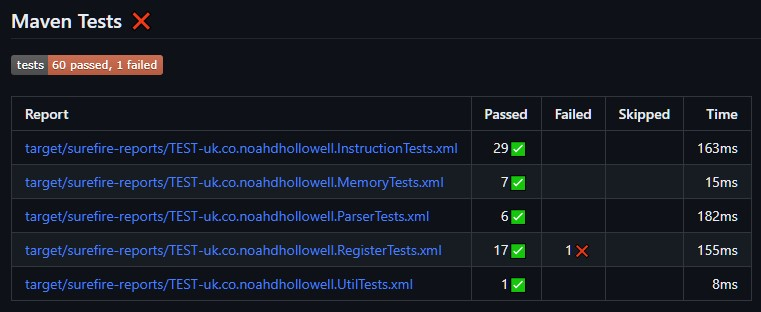
\includegraphics[width=0.8\textwidth]{dissertation/DATA/githubtest.jpg}
    \caption{Github test runner output}
    \label{fig:github_test_output}
\end{figure}

\subsubsection{Issues}
Test driven development was not without its issues. In some cases a few false positives occurred in which tests passed or failed when they shouldn't off. Fortunately, this was due to mistakes in test writing, with some test logic not calculating the correct value for the test to test against. 

A few issues also arised with the GitHub test runner. Locally the tests executed in an order that loaded instructions and cleared register and memory values in certain tests, but not all. However, the GitHub test runner ran the tests in a different order causing values to exist in the memory and registers between tests. This resulted in cascading test failures, with each additional test causing the next to fail and so on.

Thankfully, this was a simple fix to ensure that between test values were cleared completely. However, another issue quickly arose relating to the test for reading a hexadecimal value into a register. This test passes locally with correct execution, but fails on the Github runner. Specifically, the value stored in the register is expected to be \texttt{b} (11), but instead a value of 7 is returned. Despite considerable debugging and modifications, this test continues to fail on the automated runner. Whilst it is important for tests to all pass, it is the case that this test will simply be ignored as we can manually verify the underlying logic operates as expected. It is likely that the test will be removed in the future or rewritten such that it passes on the runner on Github as well as locally.

\subsection{Manual Testing}
Not all parts of the application can benefit from automated testing. The visualisation requires the physical pressing of buttons and inputting code. There may be applications that provide this functionality for Java. However for our simple \ac{UI}, a manual approach was suitable.

This approach consisted of repeatedly testing the \ac{UI} as elements were implemented. Ensuring that code ran on button clicks, animations played out smoothly in the right order, as well as ensuring elements resized properly. This testing was slower, but proved to be highly useful in order to spot visual discrepancies with resizing the window, and for spotting smaller issues with the animation sequence. Such as the animated element passing under the lines, or pushing the entire animation area off screen due to a mistake in positioning.

To ensure manual testing was rigid, a procedure was followed. This consisted of interacting with the \ac{UI} in a order in which all buttons were pressed, then menus were pressed followed by testing text inputs. Finally finishing with a cohesive script to test that all animations played correctly at varying speeds ensuring no anomalies occurred.

Further, more destructive testing was performed, with the aim of intentionally trying to break the application. This testing was performed as a worst case scenarios, in which a user may perform a combination of actions that break the application, either by accident or intentionally. This testing was sporadic with no set procedure. 

A bug that was fixed as a result of random testing occurred from the spamming of enabling and disabling of modules. If toggled fast enough it was possible for a module to be part loaded or unloaded during the next toggle which would result in the program producing a error and in some cases crashing. This was an error that would of otherwise gone unnoticed until reported by a user, and was quickly fixed by locking out the toggling checkbox until a load/unload is finished.

\section{User Feedback}
Alongside testing, user feedback was also important. It ties into our testing providing a wider set of testing environments from different devices and operating systems, as well as different interaction styles based on individual users. 

To allow for user testing a version of the final project application was packaged into a distributable Jar file that could be run on any system with Java 19 \cite{sunmicrosystems_2022_java} installed. Further, to provide a easier installation experience for fellow department students, a quick installation script was produced that downloaded the Jar and then enabled Java 19, followed by launching the application.

\begin{figure}
    \centering
    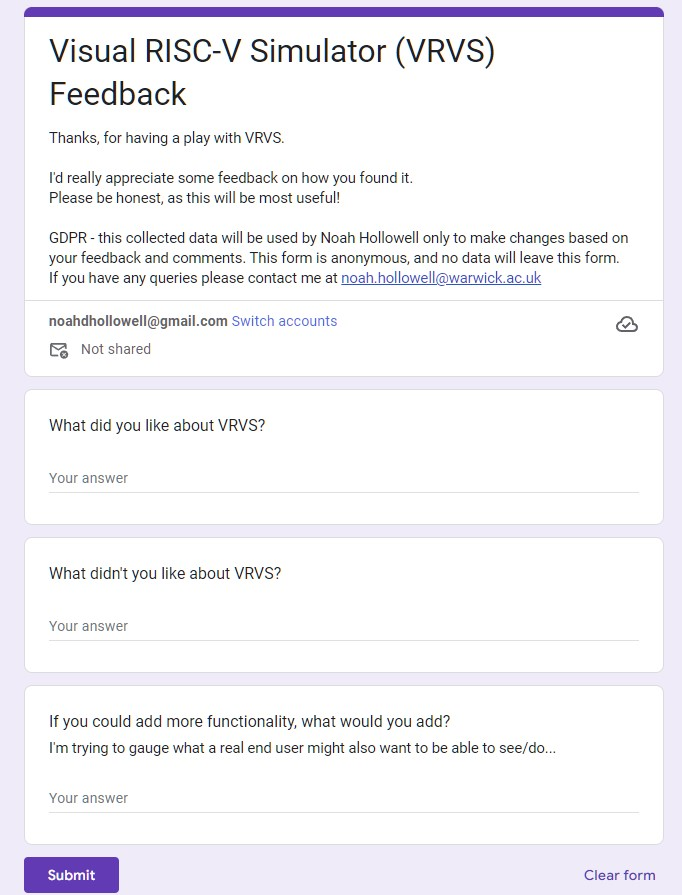
\includegraphics[width=0.8\textwidth]{dissertation/DATA/gform.jpg}
    \caption{User feedback google form}
    \label{fig:gform}
\end{figure}

Feedback was then collected via a google form (Figure \ref{fig:gform}) simply asking for what users liked, disliked and what they would find beneficial to have added.

The resulting user feedback was positive, with praise for the ease of use and functionality. The feedback also provide ample suggestions for changes and improvements, as well as identifying issues with the animation sequences and elements sizing incorrectly.

For example on user stated: "The U of ALU goes outside the orange shape and merges with the white background". This occurred when making the application widow smaller, as a result of poorly implementing the \ac{ALU} element. The element contained 3 child text elements that were spaced inside the image of the \ac{ALU}. However, as a result of doing this, when the text values holding \ac{ALU} input and output hexadecimal values became large. This caused the \ac{ALU} image to stretch in order to fit the text, which caused the image to become distorted either becoming too wide or too tall, with the white text clipping onto the background becoming hard to read.

In order to fix this issue, the text elements were separated out of the image element, being positioned individually on top of the image element, and not as children. This way the \ac{ALU} image could resize properly with the text moving respectively. Further as an additional safety measure, the text was made black, so that if it managed to overflow of, it would be clearly readable.

This user feedback was invaluable to the project, without it many of these issues wouldn't of been caught and fixed, and it also provided a mental boost during the end of development where motivation was dipping.

